\section{Problem Setup}

In this work, we focus on the particular case of autonomous corridor navigation. For this purpose we use the vanishing point algorithm \cite{VP1}, \cite{VP2} and feedback control to maintain heading parallel to the corridor and stay in the middle of it. We implement our algorithm on a $1/10^{th}$ scale car we developed. 

\subsection{The hardware}

For our experiments, we converted a Radio controlled Traxxas Rally car into an autonomous robot shown in Fig. \ref{fig:}[carFig], similar to the ones used in \cite{racecar_mit}. The computation platform is a NVIDIA Jetson TK1. The Jetson has a quad-core ARM Cortex-A15 CPU and a NVIDIA Kepler GPU. 
This setup allows us to schedule tasks on the CPU or GPU while observing the effect of this on power consumption and timing of the algorithm. 
The Jetson runs Ubuntu for Tegra as the operating system, and the algorithms are implemented using ROS \cite{ros}. The control signals for the drive and steer motor on the platform are generated by a Teensy 3.1 microcontroller running a ROS node which converts the continuous output of the control software to a PWM signal that acts as an input to the motor controller on the Traxxas. Finally, the vanishing point algorithm implemented in OpenCV \cite{opencv} gets images from a front facing Point Grey Firefly MV camera capable of recording color images at upto a resolution of 752x480 pixels and upto a frame rate of 60 FPS. 

\subsection{Vanishing point-based corridor navigation}

The Vanishing point algorithm \cite{VP1} has been used extensively in indoor settings for navigating corridors autonomously \cite{VP2, VP3} and for outdoor lane detection \cite{gallagher2002ground}. 
The algorithm outputs the horizontal distance of the frame's vanishing point and middle point from the center of the frame. 
These two measurement signals are used as feedback by the controller to center and align the robot along the corridor. 
Figure \ref{fig:vp_viz} shows a visualization of Vanishing point operating on a frame collected from our robot navigating in a corridor.

\begin{figure}[hbtp]
\centering
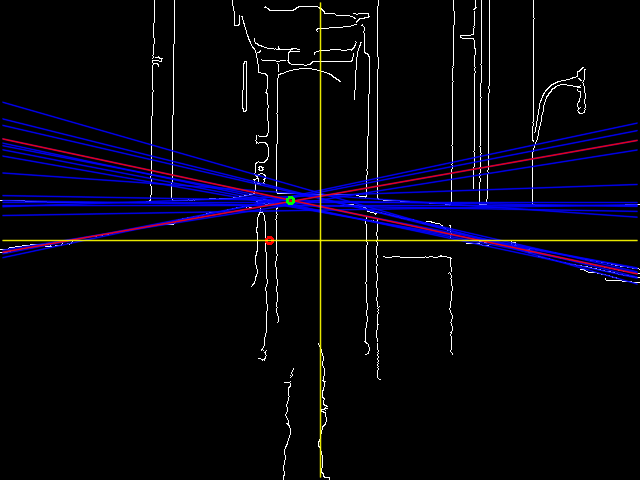
\includegraphics[width=0.46\textwidth]{Figs/vpmpimages/image_23_-30_-51.png}
\caption{Visualization of the Vanishing point algorithm. The green dot shows the vanishing point while the red dot shows the middle point.}
\label{fig:vp_viz} %diff freq same assignment}
\end{figure}


We focus on the major computational tasks that comprise the vanishing point algorithm, which are briefly explained below:

\begin{itemize}
\item Blur: A Gaussian blur is applied on the image for de-noising.
\item Edge detection: We use the Canny Edge detector to find edges in the image.
\item Hough Transform: used to detect straight lines in the image.
\item RANSAC: used to select the parallel straight lines that best describe the sides of the corridor. These lines intersect in the image plane at the Vanishing Point.
\end{itemize}


\subsection{Problem statement}
Note, on the Jetson, we can schedule any of these tasks to be run on either the CPU or the GPU as shown in Fig. \ref{fig:vanishing} In addition, we can also change the CPU and GPU frequencies during run-time, resulting in different execution times for the vanishing point algorithm and different power consumption for the Jetson. With this in mind, the problem we want to solve is that of picking the best operating mode for the perception algorithm, the vanishing point algorithm in our case, in order to minimize computation energy without overly affecting the closed loop control performance of the system. For this, we propose a two step solution and evaluate it for out problem setup. This is explained in more detail in the following sections.


